\documentclass[class=book , crop=false]{standalone}

\usepackage{import} % Required for importing other .tex docs.  (import uses everything bw Begin and End Doc)
\usepackage{float} % Required for specifying the exact location of a figure or table
\usepackage{graphicx} % Required for including images
\usepackage{wrapfig}
\usepackage[pdftex,breaklinks,colorlinks=true,linkcolor=black,citecolor=blue,urlcolor=red,linktocpage=false,pagebackref=true,filecolor=magenta]{hyperref}%http://www.tug.org/applications/hyperref/manual.html#x1-100003.6
\usepackage{cite}
\usepackage[toc,title,page]{appendix}
\usepackage{pdfpages} % enables loading a pdf into the doc
\usepackage{makeidx}
\usepackage{glossaries} % must be after hyperref
\usepackage{blindtext}
\usepackage{enumitem}
%\usepackage{caption}

%\setlist[description]{leftmargin=\parindent,labelindent=\parindent}

%\renewcommand*{\bibname}{References} % renames the bibliography

\newcommand{\HRule}{\rule{\linewidth}{0.5mm}} % Command to make the lines in the title page

\graphicspath{{img/}{GIS_ChampionSection/img/}{awardsChapter/GIS_ChampionSection/img/}{brandPart/awardsChapter/GIS_ChampionSection/img/}{img/}{pairedProgSection/img/}{methodChapter/pairedProgSection/img/}{methodPart/methodChapter/pairedProgSection/img/}{documentationSection/img/}{methodChapter/documentationSection/img/}{methodPart/methodChapter/documentationSection/img/}{docStorageOrgSection/img/}{methodChapter/docStorageOrgSection/img/}{methodPart/methodChapter/docStorageOrgSection/img/}{QGisSection/img/}{toolsChapter/QGisSection/img/}{servicePart/toolsChapter/QGisSection/img/}{ESRISection/img/}{toolChapter/ESRISection/img/}{servicePart/toolChapter/ESRISection/img/}{../../../../source/}{../../source/}{servicePart/applicationsChapter/treasurerSection/img/}}

%\setlength\parindent{0pt} % eliminates indents

\def\titlename{How This Book Works\\ \medskip\LARGE Jalape\~no}

\title{\HRule % Horizontal Line added
\\[.4cm] % space
\begin{figure}[H] % included image
\begin{center}	% centered horizontally
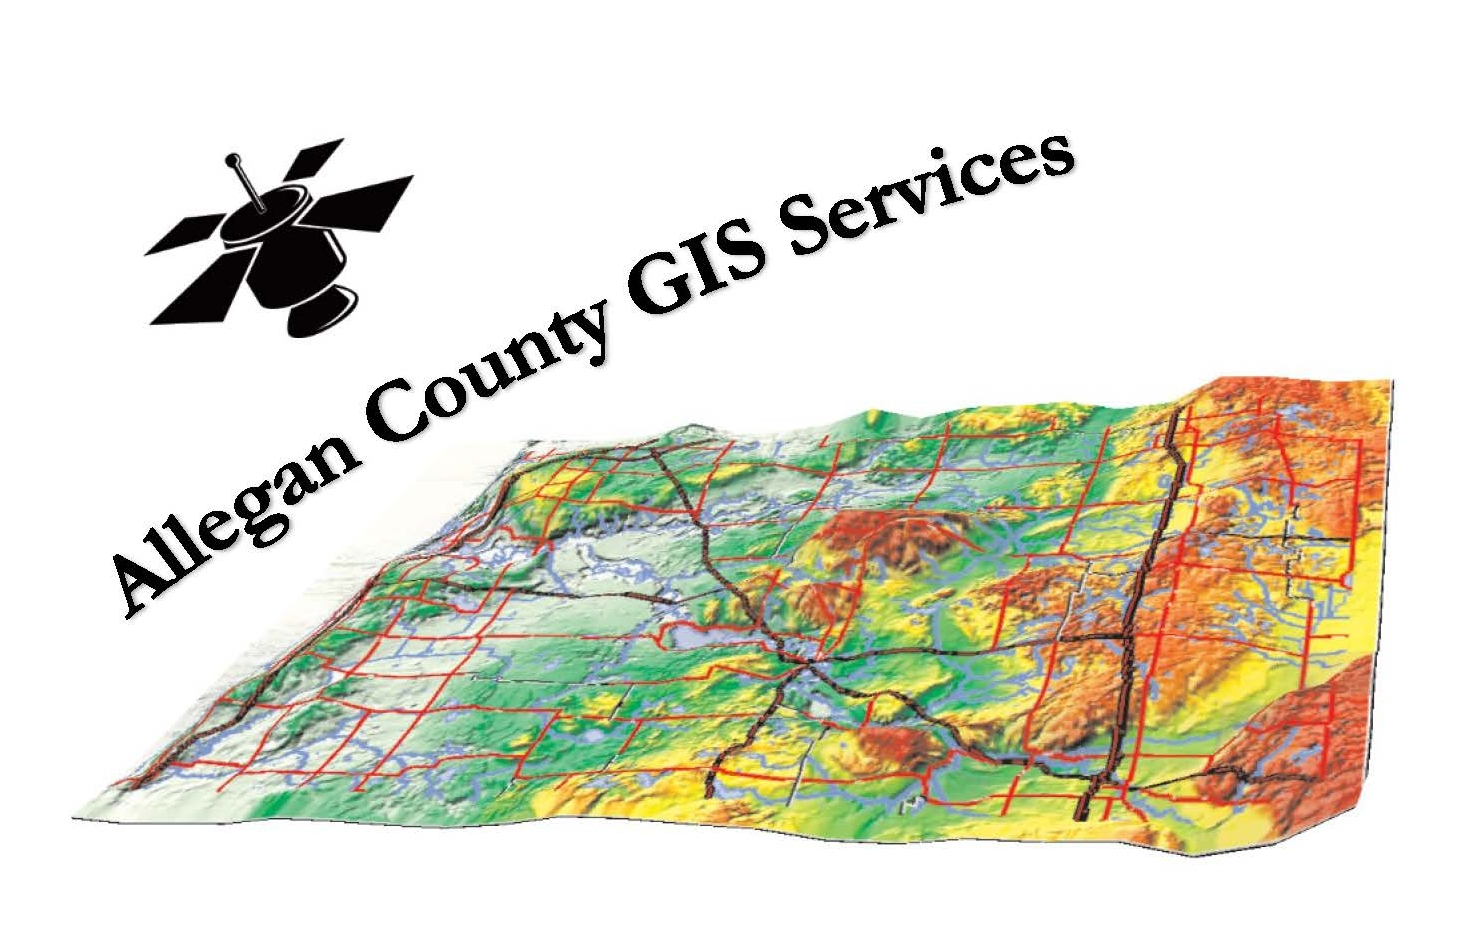
\includegraphics[scale=.45]{GIS_Logo_better.jpg}
\end{center}
\end{figure}
\Huge \bfseries \titlename \\ % Title text
\HRule \\[.4cm] % Horizontal Line added
\author{\Large Allegan County GIS \\\Large www.allegancounty.org/gis} % defines author
}  % closing brace for title

\begin{document}% Document Begins

\ifstandalone
%\frontmatter % turns off chapter numbering and uses roman numerals for page numbers
\maketitle % creates title page and blank page after title page
\tableofcontents % creates TOC and blank page
\clearpage
%\mainmatter % turns on chapter numbering, resets page numbering and uses arabic numerals for page numbers
\fi

\subsection{How This Book Works}
\subsubsection{Project General Notes:}
\begin{itemize}
\item Book folder can be renamed an moved.
\item This project is coded with relative paths from processing folder down.
\end{itemize}
\subsubsection{Project file structure:}
\begin{verbatim}
J:\LIS\GIS_Doc\book\build
\end{verbatim}
\begin{description}
\item pdf docs created by the underlying .tex docs and copied here manually.
\end{description}
\begin{verbatim}
J:\LIS\GIS_Doc\Book\source
\end{verbatim}
\begin{description}
\item images that appear in
\begin{verbatim}
\GIS_Documentation.tex
\end{verbatim}
\end{description}
\begin{verbatim}
J:\LIS\GIS_Doc\Book\processing
\end{verbatim}
\begin{description}
\item the Tex workspace.
\end{description}
\begin{verbatim}
\GIS_Documentation.tex
\end{verbatim}
\begin{description}
\item top level of documentation of type "book" in \LaTeX{}.  Where book properties and book parts are managed and chapters are imported.
\end{description}
\begin{verbatim}
\archive
\end{verbatim}
\begin{description}
\item archive copies of entire processing folder.
\end{description}
\begin{verbatim}
\brandPart
\end{verbatim}
\begin{description}
\item \LaTeX{} "book part" about the brand.
\end{description}
\begin{verbatim}
\methodsPart
\end{verbatim}
\begin{description}
\item \LaTeX{} "book part" about the methods.
\end{description}
\begin{verbatim}
\servicePart
\end{verbatim}
\begin{description}
\item \LaTeX{} "book part" about services.
\end{description}
\begin{verbatim}
\build
\end{verbatim}
\begin{description}
\item folder for temp docs when created by compiling of:
\begin{verbatim}
GIS_Documentation.tex
\end{verbatim}
\end{description}
\textbf{* Note: each level from here down has a build folder for temp Latex files like this.}
\newpage
\subsubsection{Service Book Part Detail}
relative path:
\begin{verbatim}
\processing\servicePart\toolsChapter.tex
\end{verbatim}
\begin{description}
\item  intermediate level of "book" in \LaTeX{}.  Where (service part, tool) chapter properties are managed and sections are imported.
\end{description}
\subsubsection{toolsChapter}
relative path:
\begin{verbatim}
\processing\servicePart\toolsChapter
\end{verbatim}
intermed level of "book" in \LaTeX{}.  Where book section properties are managed and subsections are imported.
\end{document}
